\documentclass[12pt]{report}
\usepackage[utf8]{inputenc}
\usepackage[russian]{babel}
%\usepackage[14pt]{extsizes}
\usepackage{listings}
\usepackage{graphicx}
\usepackage{amsmath,amsfonts,amssymb,amsthm,mathtools} 
\usepackage{pgfplots}
\usepackage{filecontents}
\usepackage{float}
\usepackage{indentfirst}
\usepackage{eucal}
\usepackage{enumitem}
%s\documentclass[openany]{book}
\frenchspacing

\usepackage{indentfirst} % Красная строка

\usetikzlibrary{datavisualization}
\usetikzlibrary{datavisualization.formats.functions}

\usepackage{amsmath}


% Для листинга кода:
\lstset{ %
	language=c,                 % выбор языка для подсветки (здесь это С)
	basicstyle=\small\sffamily, % размер и начертание шрифта для подсветки кода
	numbers=left,               % где поставить нумерацию строк (слева\справа)
	numberstyle=\tiny,           % размер шрифта для номеров строк
	stepnumber=1,                   % размер шага между двумя номерами строк
	numbersep=5pt,                % как далеко отстоят номера строк от подсвечиваемого кода
	showspaces=false,            % показывать или нет пробелы специальными отступами
	showstringspaces=false,      % показывать или нет пробелы в строках
	showtabs=false,             % показывать или нет табуляцию в строках
	frame=single,              % рисовать рамку вокруг кода
	tabsize=2,                 % размер табуляции по умолчанию равен 2 пробелам
	captionpos=t,              % позиция заголовка вверху [t] или внизу [b] 
	breaklines=true,           % автоматически переносить строки (да\нет)
	breakatwhitespace=false, % переносить строки только если есть пробел
	escapeinside={\#*}{*)}   % если нужно добавить комментарии в коде
}


\usepackage[left=2cm,right=2cm, top=2cm,bottom=2cm,bindingoffset=0cm]{geometry}
% Для измененных титулов глав:
\usepackage{titlesec, blindtext, color} % подключаем нужные пакеты
\definecolor{gray75}{gray}{0.75} % определяем цвет
\newcommand{\hsp}{\hspace{20pt}} % длина линии в 20pt
% titleformat определяет стиль
\titleformat{\chapter}[hang]{\Huge\bfseries}{\thechapter\hsp\textcolor{gray75}{|}\hsp}{0pt}{\Huge\bfseries}


% plot
\usepackage{pgfplots}
\usepackage{filecontents}
\usetikzlibrary{datavisualization}
\usetikzlibrary{datavisualization.formats.functions}

\begin{document}
	%\def\chaptername{} % убирает "Глава"
	\thispagestyle{empty}
	\begin{titlepage}
		\noindent \begin{minipage}{0.15\textwidth}
			
\includegraphics[width=\linewidth]{b_logo}
		\end{minipage}
		\noindent\begin{minipage}{0.9\textwidth}\centering
			\textbf{Министерство науки и высшего образования Российской Федерации}\\
			\textbf{Федеральное государственное бюджетное образовательное учреждение высшего образования}\\
			\textbf{~~~«Московский государственный технический университет имени Н.Э.~Баумана}\\
			\textbf{(национальный исследовательский университет)»}\\
			\textbf{(МГТУ им. Н.Э.~Баумана)}
		\end{minipage}
		
		\noindent\rule{18cm}{3pt}
		\newline\newline
		\noindent ФАКУЛЬТЕТ $\underline{\text{«Информатика и системы управления»}}$ \newline\newline
		\noindent КАФЕДРА $\underline{\text{«Программное обеспечение ЭВМ и информационные технологии»}}$\newline\newline\newline\newline\newline
		
		\begin{center}
			\noindent\begin{minipage}{1.1\textwidth}\centering
				\Large\textbf{  Отчет по лабораторной работе }\newline
				\textbf{по дисциплине <<Операционные системы>>}\newline
			\end{minipage}
		\end{center}
		
		\noindent\textbf{Тема} $\underline{\text{Буферизированный и небуферизированный ввод-вывод~~}}$\newline\newline
		\noindent\textbf{Студент} $\underline{\text{Ляпина Н.В.~~~~~~~~~~~~~~~}}$\newline\newline
		\noindent\textbf{Группа} $\underline{\text{ИУ7-62Б~~~~~~~~~~~~~~~~~~~~~~~}}$\newline\newline
		\noindent\textbf{Оценка (баллы)} $\underline{\text{~~~~~~~~~~~~~~~~~~~~~~}}$\newline\newline
		\noindent\textbf{Преподаватель} $\underline{\text{Рязанова Н.Ю.}}$\newline\newline\newline
		
		\begin{center}
			\vfill
			Москва~---~\the\year
			~г.
		\end{center}
	\end{titlepage}
\setcounter{page}{2}

\section*{Описание структур}

\begin{lstlisting}[label=first,caption=Структура FILE, language=C]
typedef struct _IO_FILE FILE;
struct _IO_FILE
{
	int _flags;		/* High-order word is _IO_MAGIC; rest is flags. */
	
	/* The following pointers correspond to the C++ streambuf protocol. */
	char *_IO_read_ptr;	/* Current read pointer */
	char *_IO_read_end;	/* End of get area. */
	char *_IO_read_base;	/* Start of putback+get area. */
	char *_IO_write_base;	/* Start of put area. */
	char *_IO_write_ptr;	/* Current put pointer. */
	char *_IO_write_end;	/* End of put area. */
	char *_IO_buf_base;	/* Start of reserve area. */
	char *_IO_buf_end;	/* End of reserve area. */
	
	/* The following fields are used to support backing up and undo. */
	char *_IO_save_base; /* Pointer to start of non-current get area. */
	char *_IO_backup_base;  /* Pointer to first valid character of backup area */
	char *_IO_save_end; /* Pointer to end of non-current get area. */
	
	struct _IO_marker *_markers;
	
	struct _IO_FILE *_chain;
	
	int _fileno;
	int _flags2;
	__off_t _old_offset; /* This used to be _offset but it's too small.  */
	
	/* 1+column number of pbase(); 0 is unknown. */
	unsigned short _cur_column;
	signed char _vtable_offset;
	char _shortbuf[1];
	
	_IO_lock_t *_lock;
	#ifdef _IO_USE_OLD_IO_FILE
};
\end{lstlisting}

\section*{Программа 1}

\begin{lstlisting}[label=first,caption=Программа 1, language=C]
#include <fcntl.h>
#include <stdio.h>

int main() {
	// have kernel open connection to file alphabet.txt
	int fd = open("alphabet.txt", O_RDONLY);
	
	// create two a C I/O buffered streams using the above connection
	FILE *fs1 = fdopen(fd, "r");
	char buff1[20];
	setvbuf(fs1, buff1, _IOFBF, 20);
	
	FILE *fs2 = fdopen(fd, "r");
	char buff2[20];
	setvbuf(fs2, buff2, _IOFBF, 20);
	
	// read a char & write it alternatingly from fs1 and fs2
	int flag1 = 1, flag2 = 2;
	while (flag1 == 1 || flag2 == 1) {
		char c;
		
		flag1 = fscanf(fs1, "%c", &c);
		if (flag1 == 1) fprintf(stdout, "%c", c);
		
		flag2 = fscanf(fs2, "%c", &c);
		if (flag2 == 1) fprintf(stdout, "%c", c);
	}
	
	return 0;
}
\end{lstlisting}

Результат работы программы: aubvcwdxeyfzghijklmnopqrst

\begin{lstlisting}[caption={\text{Программа №1 (многопоточная)}}]
#include <fcntl.h>
#include <pthread.h>
#include <stdio.h>
#define BUF_SIZE 20
#define FILENAME "alphabet.txt"

void *t1_run(void *args) {
	int *fd = (int *)args;
	FILE *fs1 = fdopen(*fd, "r");
	char buff1[BUF_SIZE];
	setvbuf(fs1, buff1, _IOFBF, BUF_SIZE);
	int flag = 1;
	char c;
	while ((flag = fscanf(fs1, "%c", &c)) == 1)
	fprintf(stdout, "%c", c);
	return NULL;
}

void *t2_run(void *args) {
	int *fd = (int *)args;
	FILE *fs2 = fdopen(*fd, "r");
	char buff2[BUF_SIZE];
	setvbuf(fs2, buff2, _IOFBF, BUF_SIZE);
	int flag = 1;
	char c;
	while ((flag = fscanf(fs2, "%c", &c)) == 1)
	fprintf(stdout, "%c", c);
	return NULL;
}

int main() {
	pthread_t t1, t2;
	int fd = open(FILENAME, O_RDONLY);
	
	pthread_create(&t1, NULL, t1_run, &fd);
	pthread_create(&t2, NULL, t2_run, &fd);
	
	pthread_join(t1, NULL);
	pthread_join(t2, NULL);
	return 0;
}
\end{lstlisting}

Результаты работы (несколько запусков программы): 
\begin{itemize}
\item abcdefghijklmnopqrstuvwxyz
\item abuvwxyzcdefghijklmnopqrst
\item aubvcwdxeyfzghijklmnopqrst
\end{itemize}

\parВ программе файл открывается \textit{один} раз системным вызовом \texttt{open}. Системный вызов \texttt{open} возвращает дескриптор файла типа \texttt{int}. Возвращенный номер \texttt{fd} -- индекс дескриптора открытого файла в таблице дискрипторов файлов процесса.
\parФункция \texttt{fdopen()} создаёт указатель на структуру \texttt{FILE}. Поле \texttt{\_fileno} в \texttt{struct \_IO\_FILE} содержит номер дескриптора, который вернула функция \texttt{open()}.
\par Функция \texttt{setvbuf()} явно задает размер буффера в 20 байт и меняет тип буферизации (для \texttt{fs1} и \texttt{fs2}) на полный.
\par При первом вызове функции \texttt{fscanf()} в цикле (для \texttt{fs1}) \texttt{buff1} будет заполнен полностью -- первыми 20 символами (буквами алфавита). \texttt{f\_pos} в структуре \texttt{struct\_file} открытого файла увеличится на 20.
\par При втором вызове \texttt{fscanf()} в цикле (для \texttt{fs2}) буффер \texttt{buff2} будет заполнен оставшимися 6 символами (начиная с \texttt{f\_pos}).

\begin{figure}[h!]
	\centering
	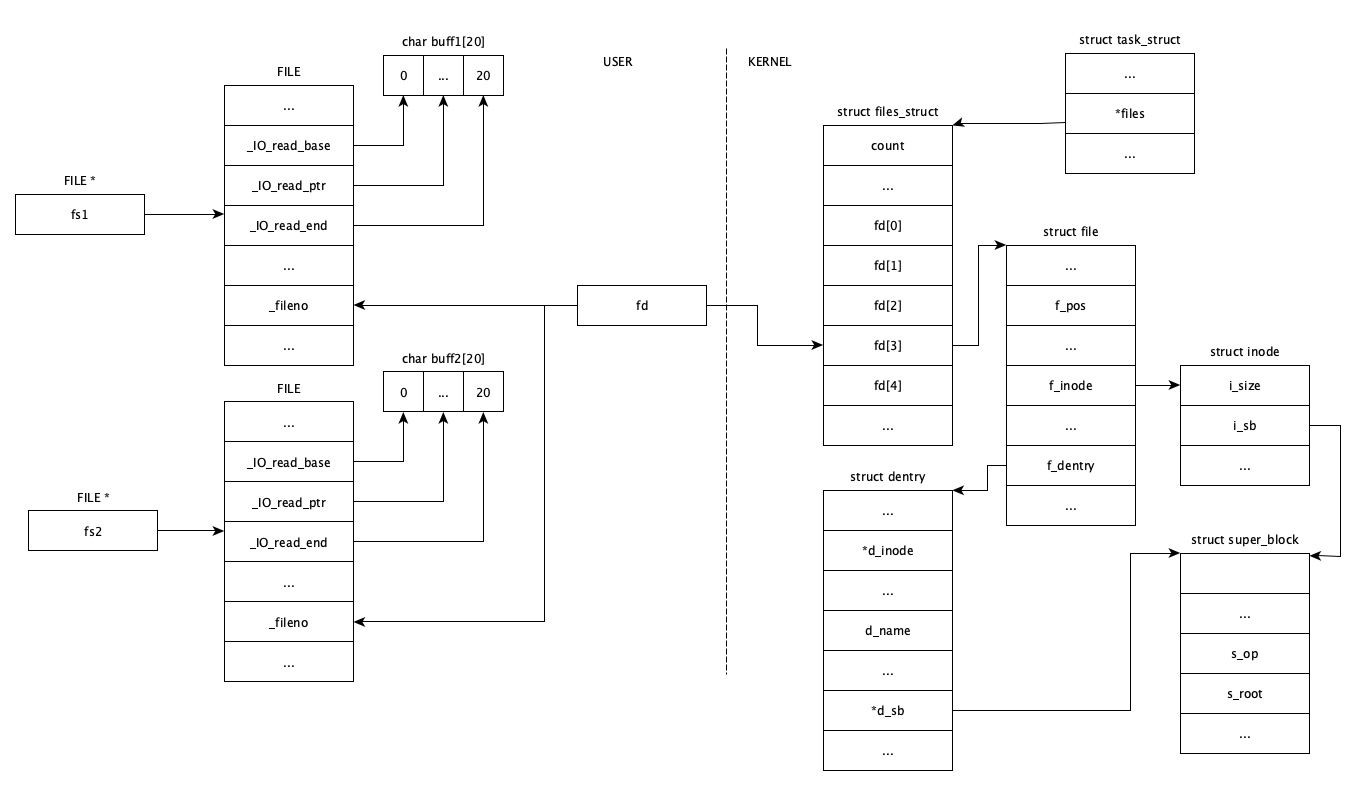
\includegraphics[scale=0.4]{1.png}
	\caption{Используемые структуры. Программа 1}
	\label{png:testing:result}
\end{figure}
\newpage

\section*{Программа 2}

\begin{lstlisting}[label=first,caption=Программа 2, language=C]
#include <fcntl.h>
#include <unistd.h>
int main() {
	int fd1 = open("alphabet.txt", O_RDONLY);
	int fd2 = open("alphabet.txt", O_RDONLY);
	char c;
	while (read(fd1, &c, 1) == 1 && read(fd2, &c, 1) == 1) {
		write(1, &c, 1);
		write(1, &c, 1);
	}
	return 0;
}
\end{lstlisting}

Результат работы: aabbccddeeffgghhiijjkkllmmnnooppqqrrssttuuvvwwxxyyzz

\begin{lstlisting}[label=first,caption=Программа 2 (многопоточная), language=C]
#include <fcntl.h> 
 #include <pthread.h> 
 #include <unistd.h> 
  
 #define FILENAME "alphabet.txt" 
  
 void *t_run(void *args) { 
     int fd = open(FILENAME, O_RDONLY); 
     int flag = 1; 
     char c; 
     while ((flag = read(fd, &c, 1)) == 1) { 
         write(1, &c, 1); 
     } 
     return NULL; 
 } 
  
 int main() { 
     pthread_t t1, t2; 
     pthread_create(&t1, NULL, t_run, NULL); 
     pthread_create(&t2, NULL, t_run, NULL); 
  
     pthread_join(t1, NULL); 
     pthread_join(t2, NULL); 
  
     return 0; 
 }
\end{lstlisting}

Результаты работы (несколько запусков программы): 
\begin{itemize}
	\item aabcdbefcgdheifjgkhlimjnkolpmqnrosptqurvswtxuyvzwxyz
	\item aabbcdcedfefgghhiijjkkllmmnnooppqqrrssttuuvvwwxxyyzz
	\item aabbccddeeffgghihjijkkllmmnnopoqprqsrtsutvuwvxwyxzyz
\end{itemize}


\parФункция \texttt{open()} создает файловый дескриптор, два раза для одного и того же файла, поэтому в программе существует два дескриптора открытого файла \texttt{struct file}, но ссылающиеся на один и тот же \texttt{struct inode}.
\parИз-за того что структуры разные (у каждой структуры свое поле \texttt{f\_pos}), посимвольная печать дважды выведет содержимое файла в формате <<\texttt{aabbcc...}>> (в случае однопоточной реализации).
\parВ случае многопоточной реализации, потоки выполняются с разной скоростью и символы перемешаются.


\begin{figure}[h!]
	\centering
	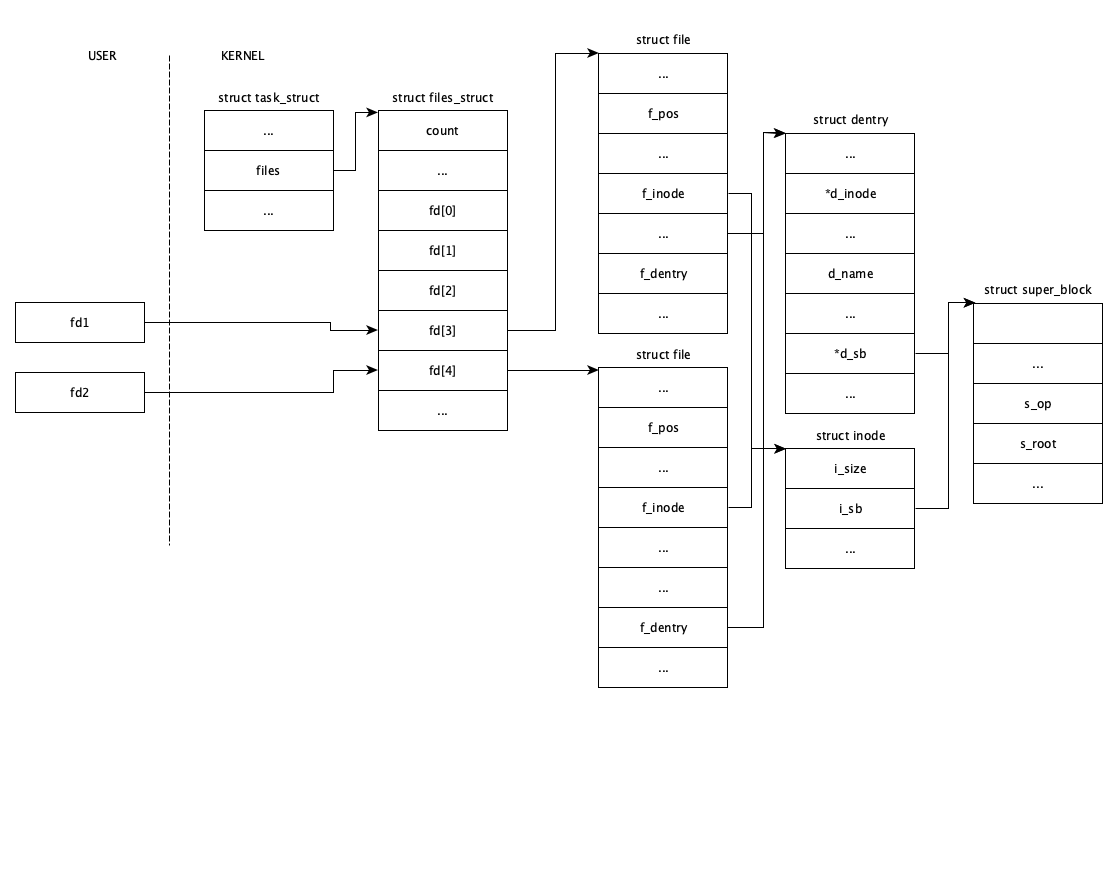
\includegraphics[scale=0.4]{2.png}
	\caption{Используемые структуры. Программа 2}
	\label{png:testing:result}
\end{figure}
\newpage

\section*{Программа 3}

\begin{lstlisting}[label=first,caption=Программа 3, language=C]
#include <fcntl.h>
#include <stdio.h>
#include <unistd.h>

#define FILENAME "out.txt"

int main() {
	FILE *f1 = fopen(FILENAME, "w");
	FILE *f2 = fopen(FILENAME, "w");
	
	for (char c = 'a'; c <= 'z'; c++) {
		if (c % 2) {
			fprintf(f1, "%c", c);
		} else {
			fprintf(f2, "%c", c);
		}
	}
	
	fclose(f1);
	fclose(f2);
	
	return 0;
}
\end{lstlisting}

Результат работы: bdfhjlnprtvxz

\begin{lstlisting}[label=first,caption=Программа 3 (многопоточная), language=C]
#include <fcntl.h>
#include <pthread.h>
#include <stdio.h>
#include <unistd.h>

#define FILENAME "out.txt"

void *t1_run(void *args) {
	FILE *f = fopen(FILENAME, "w");
	
	for (char c = 'a'; c <= 'z'; c += 2) {
		fprintf(f, "%c", c);
	}
	
	fclose(f);
	
	return NULL;
}

void *t2_run(void *args) {
	FILE *f = fopen(FILENAME, "w");
	
	for (char c = 'b'; c <= 'z'; c += 2) {
		fprintf(f, "%c", c);
	}
	
	fclose(f);
	
	return NULL;
}

int main() {
	pthread_t t1, t2;
	pthread_create(&t1, NULL, t1_run, NULL);
	pthread_create(&t2, NULL, t2_run, NULL);
	
	pthread_join(t1, NULL);
	pthread_join(t2, NULL);
	
	return 0;
}
\end{lstlisting}

Результаты работы (несколько запусков программы): 
\begin{itemize}
	\item acegikmoqsuwy
	\item bdfhjlnprtvxz
\end{itemize}

\parФайл открывается на запись два раза функцией \texttt{fopen()}.
\parИз-за того \texttt{f\_pos} независимы для каждого дескриптора файла, запись в файл будет производится с нулевой позиции.
\parФункция \texttt{fprintf()} предоставляет буферизованный вывод.
\parИзначально информация пишется в буфер, а из буфера в файл если произошло одно из
событий:
\begin{enumerate}
	\item буффер заполнен
	\item вызвана функция \texttt{fclose()}
	\item вызвана функция \texttt{fflush()}
\end{enumerate}
\parВ случае нашей программы, информация в файл запишется в результате вызова функции \texttt{fclose()}. При вызове fclose() для fs1 буфер для fs1 записывается в файл. При вызове fclose() для fs2, все содержимое файла затирается, а в файл записывается содержимое буфера для fs2. В итоге произошла потеря данных, в файле окажется только содержимое буфера для fs2. Чтобы этого избеать, необходимо использовать флаг O\_APPEND. Если этот флаг установлен, первая запись в файл не теряется. 

\begin{figure}[h!]
	\centering
	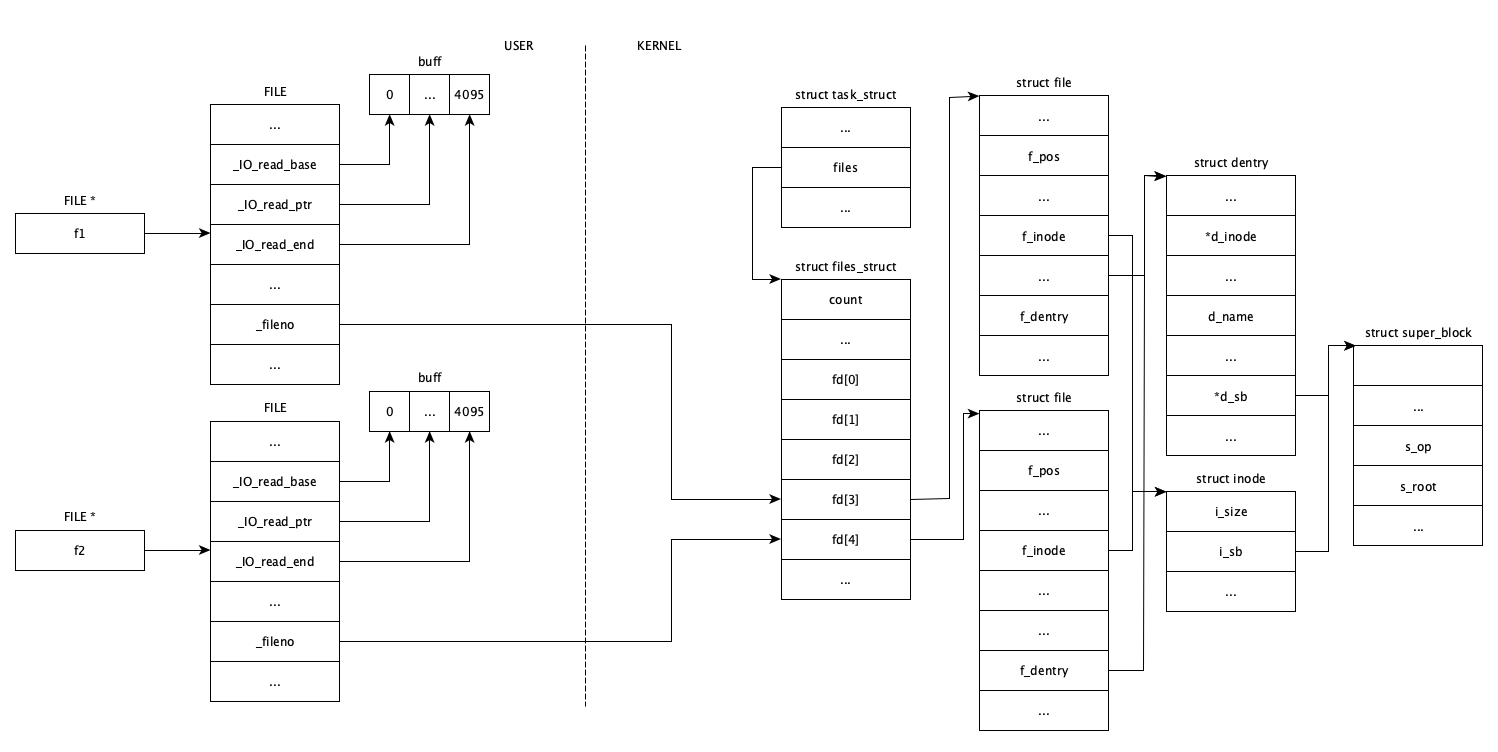
\includegraphics[scale=0.35]{3.png}
	\caption{Используемые структуры. Программа 3}
	\label{png:testing:result}
\end{figure}
\newpage

\begin{lstlisting}[label=open,caption={Программа 3 (с open, read, write)}, language=C]
#include <fcntl.h>
#include <stdio.h>
#include <unistd.h>

#define FILENAME "out.txt"

int main() {
	int f1 = open(FILENAME, O_WRONLY | O_CREAT);
	int f2 = open(FILENAME, O_WRONLY | O_CREAT);
	
	for (char c = 'a'; c <= 'z'; c++) {
		if (c % 2) {
			write(f1, &c, 1);
		} else {
			write(f2, &c, 1);
		}
	}
	
	close(f1);
	close(f2);
	return 0;
}
\end{lstlisting}

Результат работы: bdfhjlnprtvxz

\begin{lstlisting}[label=first,caption={Программа 3 (с open, read, write) (многопоточная)}, language=C]
#include <fcntl.h>
#include <pthread.h>
#include <stdio.h>
#include <unistd.h>

#define FILENAME "out.txt"

void *t1_run(void *args) {
	int f = open(FILENAME, O_WRONLY | O_CREAT);
	
	for (char c = 'a'; c <= 'z'; c += 2) {
		write(f, &c, 1);
	}
	
	close(f);
	
	return NULL;
}

void *t2_run(void *args) {
	int f = open(FILENAME, O_WRONLY | O_CREAT);
	
	for (char c = 'b'; c <= 'z'; c += 2) {
		write(f, &c, 1);
	}
	
	close(f);
	
	return NULL;
}

int main() {
	pthread_t t1, t2;
	pthread_create(&t1, NULL, t1_run, NULL);
	pthread_create(&t2, NULL, t2_run, NULL);
	pthread_join(t1, NULL);
	pthread_join(t2, NULL);
	return 0;
}
\end{lstlisting}

Результаты работы (несколько запусков программы): 
\begin{itemize}
	\item acegikmoqsuwy
	\item bdfhjlnprtvxz
\end{itemize}

\parСистемный вызов \texttt{write} записывает данные в файл сразу после вызова, а отличие от библиотечной функции \texttt{fprintf()}, которая сначала записывает данные в буфер, и только после вызова функции \texttt{fclose()} -- в файл. 
\parПрограмма, представленная в листинге \ref{open}, работает следующим образом. Системный вызов \texttt{open} возвращает индекс в массиве открытых файлов процесса, причем каждый раз возвращается новый индекс, даже если открывается один и тот же файл. Затем при системном вызове \texttt{write} для f1 данные сразу записываются в файл, но из-за того, что при системной вызове \texttt{open} указатель устанавливается в начало файла, следующий системный вызов \texttt{write} для f2 затирает данные предыдущего вызова.
\parДля предотвращения затирания данных нужно использовать флаг O\_APPEND в качестве аргумента системного вызова \texttt{open}. Этот флаг устанавливает указатель на конец файла перед каждым вызовом \texttt{write}.


\end{document}